%!Tex Program = xelatex
\documentclass[11pt]{article}
\usepackage{fontspec}
\usepackage{xeCJK}
\usepackage{graphicx}
\usepackage{float}
\setmainfont[Mapping=tex-text,BoldFont=WenQuanYi Zen Hei]{WenQuanYi Zen Hei}
\begin{document}
\section{总体设计}
\subsection{功能目标}
    \begin{itemize}
        \item 将软板卡模拟成ips板卡,与rps交互
        \item 软板卡可以完成放音功能,并支持指定放音文件名、循环、循环间隔、最大
            时长、放音外部中止等关键特性
        \item 板卡可以完成收号功能,并支持正常收号、整体超时、首号超时、号间超时
            外部中止,结束键判断,收号最大最小长度判断等关键特性
        \item 软板卡支持放音收号的功能组合
        \item 软板卡支持多路并发的进行以上功能
        \item 软板卡可以记录日志
        \item 软板卡可以统计自系统运行以来的基本信息
        \item 软板卡在发生故障时可以发送告警信息
        \item 软板卡的日志,统计,告警功能可以与公司即有系统进行对接
    \end{itemize}
\subsection{性能目标}
    以HMP的价格为基础,通过对硬件及相关软件的成本核算,软板卡达到单机400路以上,
    即可以节约总体成本。所以,性能要求为在cpu为"Quad core Intel Core i5-2400
    1600.00 MHz",内存为3GB的机器上,支持400路以上并发。

\subsection{总体处理架构}
    软板卡以session为基本单位向rps提供媒体能力。session是软板卡的一个管理单位,
    所有具体的功能实体,均以session为范围界限,进行管理。每一个session的内部,
    均可以独立且并行的运行若干功能实体,如放音操作、收号操作等。目前一个session
    只允许同时运行一个放音操作和一个收号操作,未来可以根据需求,增加新的功能实
    体如录音,视频播放等,也可以增加操作实体的并发数量,如同时播放多个音频。
    session之间数据保持独立,session以唯一标识进行识别。

    软板卡与rps之间,使用icp消息进行信息传递,每一次消息收发称为一次交互,其中,
    发起一次交互的消息称为请求,返回请求消息的处理反馈的消息,称为结果。
    session通过特殊的交互创建和销毁,并在整个生命周期期间,与rps进行操控有关的多
    次交互。交互的请求处理和结果返回是异步的,所以软板卡在处理一次交互的过程中,
    可以接收新的交互,并且不保证结果按请求的顺序返回。比如放音交互,板卡在收到
    放音请求后开始放音,之后又收到停止放音的交互,于是停止放音并返回两个交互
    的处理结果,但是,尽管停止放音的请求在后,停止放音的结果有可能比放音结束的
    结果更早返回。

    软板卡内部,针对每一个session,创建一个worker。除特殊的创建销毁交互外,其他
    所有的交互均根据需要创建若干个erlang进程,每个进程向worker发送一条控制指令,
    并被worker阻塞,直到收到结果后,向rps返回处理结果。

    参见message.pdf

\clearpage
\subsection{总体运行架构及主要功能模块说明}
    ocarina总体运行架构由三部分组成:总控模块,功能处理模块和信息管理模块。总控
    模块直接收发与rps交互的icp消息,在收到特殊交互时,向系统内部申请或是释放资
    源。功能处理模块主要处理实际的请求,并返回处理结果。总控模块和功能处理模块
    均可以根据需要向信息处理模块发送内部消息,如:创建新的worker,播放名字为
    audio.wav的文件。消息可以是以debug,日志,统计等为目的的任何信息,
    特别地,告警信息也会发送到消息管理模块。消息管理模会根据消息种类,来决定
    信息的处理方式,如发送至告警服务器或是进行日志记录。参见图片struct。

\begin{figure}[h!]
    \centering
        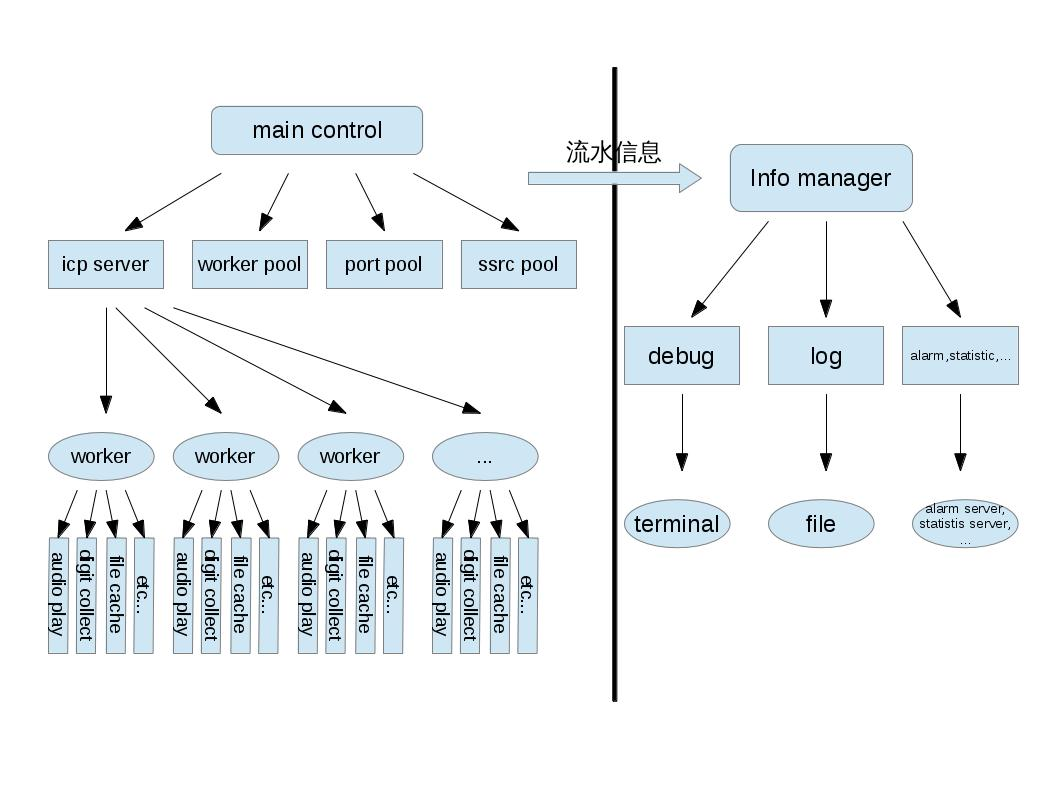
\includegraphics[width=1.0\textwidth]{struct.jpg}
    \caption{struct}
\end{figure}

    总控模块(main control):负责ocarina的初始化,监听端口,基本的icp消息编解码,及针对特殊交
    互进行资源的分配和回收等功能。总控模块主要由worker pool, ssrc pool, port
    pool,及icp server组成。

    功能处理模块(worker):每一个功能处理,将在收到创建交互的时候,实例化为一个worker,即
    每一个session对应一个worker。每一个worker独立运行,worker之间不共享信息。
    Worker内部将会记录与session相关的信息,如ssrc的id,对外发送数据的端口等。
    同时,每一个worker内部会启动若干个功能实例,如放音实例,用于将音频数据从指
    定端口发送到指定地址;或收号实例,用于从指定端口收号;或两者同时工作。worker
    在收到请求后,会阻塞请求的进程,并在处理完成后,向进程返回处理结果。

    信息管理模块(info manager):信息管理模块由一个信息集合器和若干信息处理器组成。系统运行时,
    可以动态的向信息集合器注册或注销信息处理器。信息处理器注册之后,就会收到所
    有发送到信息集合器的信息。整个系统运行过程之中,系统内所有组件,均向信息集合
    器发送信息,信息集合器将全部信息转发给所有注册了的信息处理器,信息处理器根据
    自身的功能和需求,针对特别的信息进行处理,并忽略其他信息。比如日志处理器,
    将针对所有日志信息,记录到日志文件中,并忽略所有的告警信息,以及其他的debug
    信息等。
\end{document}
